%Autor: Simon Walker
%Version: 1.0
%Datum: 10.11.2019

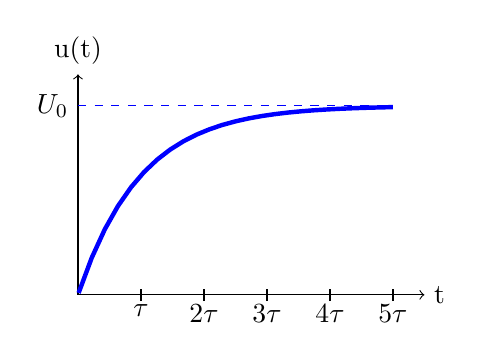
\begin{tikzpicture}[xscale=0.8, yscale=0.8]
	%\draw[help lines] (0,0) grid (6,4);
	\normalsize
	
	\draw [<->] (0, 3.5) -- (0, 0) -- (5.5, 0);
	\node [right] at (5.5, 0) {t};
	\node [above] at (0, 3.5) {u(t)};
	
	\draw (1, -0.1) --  (1, 0.1);
	\node [below] at (1, 0) {$\tau$};
	\draw (2, -0.1) --  (2, 0.1);
	\node [below] at (2, 0) {$2\tau$};
	\draw (3, -0.1) --  (3, 0.1);
	\node [below] at (3, 0) {$3\tau$};
	\draw (4, -0.1) --  (4, 0.1);
	\node [below] at (4, 0) {$4\tau$};
	\draw (5, -0.1) --  (5, 0.1);
	\node [below] at (5, 0) {$5\tau$};
	
	\draw [dashed, blue] (0, 3) -- (5, 3);
	\node [left] at (0,3) {$U_0$};
	\draw[blue, ultra thick, domain=0.01:5] plot (\x, {3*(1-e^(-\x))});
	
\end{tikzpicture}
